\section{Justificación}

TASMC te va a proporcionar listados de hoteles, vuelos y objetos que debes considerar en tu equipaje y facilidades para generar un itinerario, hasta este punto es prácticamente lo mismo que te ofrecen otras aplicaciones. Sin embargo, existen dos novedades que nos diferencian de dichas aplicaciones:

\begin{enumerate}
	\item La ruta más conveniente para llegar al aeropuerto que se sugerirá dependiendo la distancia del  trayecto utilizando un servicio externo de Geolocalización, esto se puede obtener con otras aplicaciones dedicadas específicamente a rutas, nosotros lo brindamos en una misma aplicación dedicada a la gestión integral del viaje.
	\item El punto más novedoso de nuestro sistema es la "Localización en Interiores", esta rama de la localización aun no es tan utilizada por diferentes razones, una de ellas es que el GPS carece de un funcionamiento tan eficaz en interiores comparándolo con el desempeño en exteriores. Nuestro sistema será el primero que implemente la localización en interiores para el AICM.  
\end{enumerate}

Nuestro proyecto beneficiará a todos los viajeros aéreos del AICM, independientemente del tipo de viaje. Por ejemplo, un viajero que no visita constantemente el aeropuerto le será de mucha utilidad la localización en interiores ya que le facilitará encontrar su sala de abordaje de una manera eficaz. Por otro lado, una persona que visita constantemente el AICM puede ubicarse con facilidad pero de ninguna manera puede perder su vuelo lo cual se evitará utilizando nuestra sugerencia de rutas al aeropuerto. Finalmente, lo que se quiere es que el usuario de nuestro sistema tenga una mejor planeación, organización y control de su viaje, además de un ahorro de tiempo, combustibles y dinero, lo que se logrará con la información que el sistema proporcionará a través del móvil.
 
Finalmente, con el desarrollo de este trabajo terminal se busca aprovechar y hacer frente a las siguientes observaciones:

\begin{itemize}
	\item El turismo en México es una actividad fundamental en el desarrollo económico del país.
	\item El turista se enfrenta a un problema que puede dificultar su viaje al no tener bien organizado el mismo.
\end{itemize}

El sistema estará orientado a dispositivos móviles debido al constante crecimiento en el número de usuarios de este tipo de dispositivos y al acelerado avance tecnológico en los sistemas móviles, en particular, el sistema estará disponible para dispositivos móviles con el sistema operativo Android, esto debido a que actualmente es el sistema operativo líder en el mercado (ver Figura \ref{fig:moviles})\cite{moviles} y ofrece una mayor flexibilidad para el desarrollo de aplicaciones en comparación con sus principales competidores.

\begin{figure}[htbp]
	\centering
		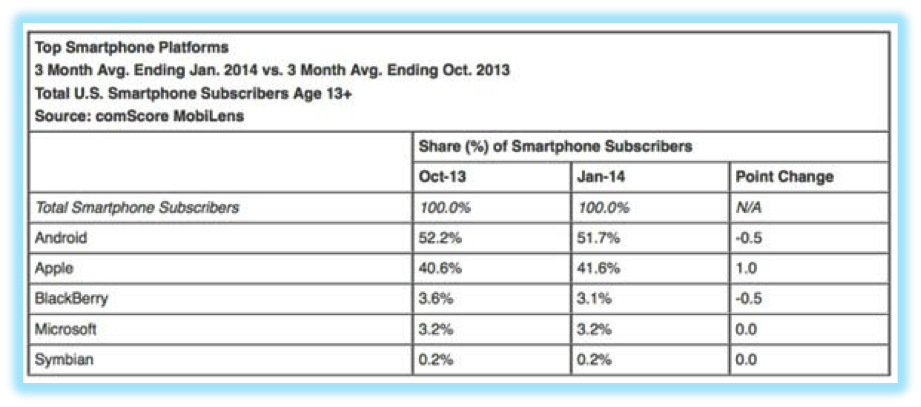
\includegraphics{Figuras/moviles.png}
		\rule{35em}{0.5pt}
	\caption[Mercado de los S.O. Móviles]{Presencia Actual en el Mercado de los S.O. Móviles}
	\label{fig:moviles}
\end{figure}